\documentclass{article}[18pt]
\ProvidesPackage{format}
%Page setup
\usepackage[utf8]{inputenc}
\usepackage[margin=0.7in]{geometry}
\usepackage{parselines} 
\usepackage[english]{babel}
\usepackage{fancyhdr}
\usepackage{titlesec}
\hyphenpenalty=10000

\pagestyle{fancy}
\fancyhf{}
\rhead{Sam Robbins}
\rfoot{Page \thepage}

%Characters
\usepackage{amsmath}
\usepackage{amssymb}
\usepackage{gensymb}
\newcommand{\R}{\mathbb{R}}

%Diagrams
\usepackage{pgfplots}
\usepackage{graphicx}
\usepackage{tabularx}
\usepackage{relsize}
\pgfplotsset{width=10cm,compat=1.9}
\usepackage{float}

%Length Setting
\titlespacing\section{0pt}{14pt plus 4pt minus 2pt}{0pt plus 2pt minus 2pt}
\newlength\tindent
\setlength{\tindent}{\parindent}
\setlength{\parindent}{0pt}
\renewcommand{\indent}{\hspace*{\tindent}}

%Programming Font
\usepackage{courier}
\usepackage{listings}
\usepackage{pxfonts}

%Lists
\usepackage{enumerate}
\usepackage{enumitem}

% Networks Macro
\usepackage{tikz}


% Commands for files converted using pandoc
\providecommand{\tightlist}{%
	\setlength{\itemsep}{0pt}\setlength{\parskip}{0pt}}
\usepackage{hyperref}

% Get nice commands for floor and ceil
\usepackage{mathtools}
\DeclarePairedDelimiter{\ceil}{\lceil}{\rceil}
\DeclarePairedDelimiter{\floor}{\lfloor}{\rfloor}

% Allow itemize to go up to 20 levels deep (just change the number if you need more you madman)
\usepackage{enumitem}
\setlistdepth{20}
\renewlist{itemize}{itemize}{20}

% initially, use dots for all levels
\setlist[itemize]{label=$\cdot$}

% customize the first 3 levels
\setlist[itemize,1]{label=\textbullet}
\setlist[itemize,2]{label=--}
\setlist[itemize,3]{label=*}

% Definition and Important Stuff
% Important stuff
\usepackage[framemethod=TikZ]{mdframed}

\newcounter{theo}[section]\setcounter{theo}{0}
\renewcommand{\thetheo}{\arabic{section}.\arabic{theo}}
\newenvironment{important}[1][]{%
	\refstepcounter{theo}%
	\ifstrempty{#1}%
	{\mdfsetup{%
			frametitle={%
				\tikz[baseline=(current bounding box.east),outer sep=0pt]
				\node[anchor=east,rectangle,fill=red!50]
				{\strut Important};}}
	}%
	{\mdfsetup{%
			frametitle={%
				\tikz[baseline=(current bounding box.east),outer sep=0pt]
				\node[anchor=east,rectangle,fill=red!50]
				{\strut Important:~#1};}}%
	}%
	\mdfsetup{innertopmargin=10pt,linecolor=red!50,%
		linewidth=2pt,topline=true,%
		frametitleaboveskip=\dimexpr-\ht\strutbox\relax
	}
	\begin{mdframed}[]\relax%
		\centering
		}{\end{mdframed}}



\newcounter{lem}[section]\setcounter{lem}{0}
\renewcommand{\thelem}{\arabic{section}.\arabic{lem}}
\newenvironment{defin}[1][]{%
	\refstepcounter{lem}%
	\ifstrempty{#1}%
	{\mdfsetup{%
			frametitle={%
				\tikz[baseline=(current bounding box.east),outer sep=0pt]
				\node[anchor=east,rectangle,fill=blue!20]
				{\strut Definition};}}
	}%
	{\mdfsetup{%
			frametitle={%
				\tikz[baseline=(current bounding box.east),outer sep=0pt]
				\node[anchor=east,rectangle,fill=blue!20]
				{\strut Definition:~#1};}}%
	}%
	\mdfsetup{innertopmargin=10pt,linecolor=blue!20,%
		linewidth=2pt,topline=true,%
		frametitleaboveskip=\dimexpr-\ht\strutbox\relax
	}
	\begin{mdframed}[]\relax%
		\centering
		}{\end{mdframed}}
\lhead{Computer Systems - Dr Magnus Bordewich}


\begin{document}
\begin{center}
\underline{\huge Machine Architecture Introduction and LMC Model}
\end{center}
\section{History of Computers}
\begin{itemize}
\item Pre 1950s - meant a person in a room doing calculations
\item 1871 - Babbage's analytical engine - advanced mechanical calculator that could be programmed in a limited sense. Programmes made by Ada Lovelace
\item 1950s-1960s - Curta Calculator - sophisticated mechanical calculator
\end{itemize}
\subsection{Enigma}
Evolved from mechanical to electromechanical in the emigma machine.\\
Rotor wheels at the heart of the device physically set at the start, then rotated as typed. Wires within wheels to increase difficulty to decrypt without the rotors.\\
\\
The enigma is a \textbf{polyalphabetic substitution cipher} based on electromechanical rotors that changed the substitution cypher after each letter.\\
This would have been unbreakable if better procedures had been followed during use
\subsection{The BOMBE}
Created by Turing and Colleagues. Tackled the enigma machine. Developed speed, efficiency and reliability.
\subsection{Colossus}
More sophisticated than the BOMBE, used against the Lorenz cypher. This was programmable, making it easier to input the new settings each day.
\subsection{Turing's definition of a computer}
\begin{center}
"The idea behind digital computers may be explained by saying that these machines are intended to carry out any operations which could not be done by a human computer" - Alan Turing
\end{center}
\subsection{A Turing Machine}
An abstract mathematical model of computation. Manipulations of 0s and 1s on an infinite strip of paper. Head can make manipulations on the viewed square and move left and right. Shown that all things that could be computed by a more complicated model could be computed by a Turing machine. This is a universal computer
\subsection{1948 - Manchester Baby}
Winner of the race to build the first \textbf{Turing complete} computer. Impractical to use and program
\subsection{1952 - IAS Machine}
A more practical Turing Complete computer, team behind it headed by von Neumann. Program not hard wired into machine, instead in storage.
\subsection{von Neumann Architecture}
Program made part of data\\
\\
Developed by the EDVAC design team for the US Army.\\
The main elements of a computer are virtually unchanged from this:
\begin{itemize}
\item Memory holds both programs and data - "Stored Program Concept" - this means machine doesn't need to be rewired for different programs
\item Memory is addressed linearly - memory read in order, find what is a program and perform it
\item Instructions executed sequentially (unless a branch or reset occurs)
\end{itemize}
\section{LMC Model of Computing}
\begin{center}
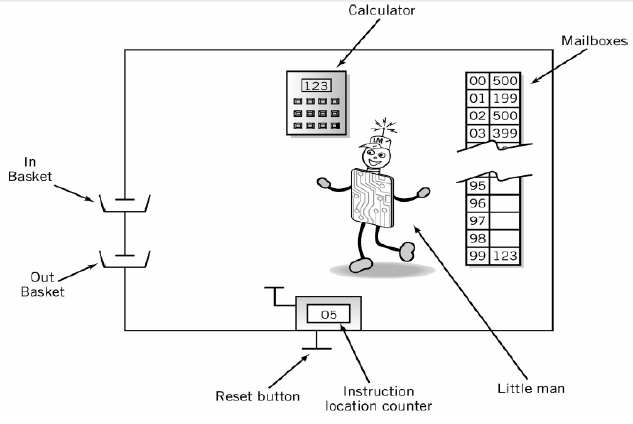
\includegraphics[width=10cm]{LMC.png}
\end{center}
Essential features:
\begin{itemize}
\item \textbf{Mailboxes} - Have 2 digit addresses so a maximum of 100 mailboxes. Each mailbox contains a slip of paper with 3 digits on it - no more. Store data in these mailboxes
\item \textbf{Calculator} - Can only display 3 digits, has 0-9,+,- and a flag for negative results. Calculator will loop after 999
\item \textbf{2 digit counter} - One button to increment the number, one external one to reset it to zero - tells the man which mailbox to look at next. Each time read, man increments it by 1
\item \textbf{Input and Output Trays}\begin{itemize}
\item The user can put slips with 3 digits on the \textbf{input} tray, to be read when the little man next looks at this tray
\item The little man can write 3 digit notes and put them in the \textbf{output} tray, to be read by the user  - whenever number read from input tray, put into calculator
\end{itemize}
\end{itemize}
The process, the little man:
\begin{itemize}
\item Starts by looking at the counter for a mailbox number X
\item The man increments the counter by 1
\item The man goes to mailbox X and reads what is written on the slip of paper in the mailbox - 3 digits
\item The man takes the appropriate action depending on those digits
\item The man starts again
\end{itemize}
\subsection{Instruction set}
The little man will read the 3 digit message in the mailbox he is sent to, for example 584\\
The first digit is the instruction (5)\\
The second and third digits are another mailbox number (84)\\
The instruction part is also known as an \textbf{op code} (operation code)\\
\\
The power of this architecture is that a number in a mailbox can be treated either as a instruction or data
\subsubsection{Example Instructions}
\textbf{op code 5 - LOAD}\\
LOAD, so the man would go to the mailbox address specified, read the 3 digit number at that address, then go to the calculator and enter that number in\\
\\
\textbf{op code 3 - STORE}\\
Go to the calculator and note that 3 digit number displayed, then go to the mailbox address specified and enter that number on a new slip of paper\\
\\
\textbf{op code 1 - ADD}\\
Go to the mailbox address specified, read the 3 digit number at that address, then go to the calculator and add the number to the number already on the calculator\\
\\
\textbf{op code 2 - SUBTRACT}\\
Go to the mailbox address specified, read the 3 digit number at that address, then go to the calculator and subtract the number from the number already on the calculator\\
\\
\textbf{op code 9 - INPUT/OUTPUT}\\
\textbf{Input/Read - op code 9 address 01} - Go to the IN tray, read the 3 digit number there, then go to the calculator and enter the number in\\
\textbf{Output/Print - op code 9 address 02} - Go to the calculator, read the 3 digit number there, then go to the OUT tray and leave a slip of paper there with that number on it\\
\\
\textbf{op code 0 - BREAK}
The little man has a rest
\subsubsection{Extended Instruction Set}
\textbf{op code 6 - BRANCH}\\
Set the counter to the 2 digits specified in the address, and start fetch of instruction from this new address\\
\\
\textbf{op code 7 - BRANCH on ZERO}\\
Go to the counter and read the 3 digit number. If it is zero, set the counter to the 2 digits specified in the address, and start fetch of instruction. Otherwise continue with the next instruction as normal.\\
\\
\textbf{op code 8 - BRANCH on POSITIVE}\\
Go to the calculator and read the 3 digit number. If it is positive (including zero), set the counter to the 2 digits specified in the address, and start fetch of instruction, otherwise continue with the next instruction as normal\\
\\
BRANCH can also be used to form loops by branching backwards
\subsubsection{Instruction set overview}
\textbf{Machine Control}\\
op code 0 - BREAK\\
\\
\textbf{Arithmetic}\\
op code 1 - ADD\\
op code 2 - SUBTRACT\\
\\
\textbf{Data Movement}\\
op code 3 - STORE\\
op code 5 - LOAD\\
\\
\textbf{Branching}\\
op code 6 - BRANCH\\
op code 7 - BRANCH on ZERO\\
op code 8 - BRANCH on POSITIVE\\
\\
\textbf{Input/Output}
op code 901 - INPUT\\
op code 902 - OUTPUT



\subsection{LMC fetch execute cycle}
There are two essential phases of the LMC instruction cycle:
\begin{itemize}
\item \textbf{fetch} - in which the little man finds the instruction to execute
\item \textbf{execute} - in which the little man performs the work specified in the instruction
\end{itemize}
\subsubsection{Fetch}
\begin{itemize}
\item The man goes to the counter and reads the address there
\item The man goes to the mailbox at that address and reads the 3 digit number in the mailbox
\end{itemize}
\subsubsection{Execute}
\begin{itemize}
\item The man remembers the target address
\item The man goes to the calculator and reads the 3 digits
\item The man goes to the mailbox at the remembered address
\item The man writes the 3 digits on a slip at that address
\item The man goes to the counter and increments it
\end{itemize}
The man needs to \textbf{remember} an address and a 3 digit value
\subsection{Potential errors}
If data is stored without a halt beforehand, the data will be executed, causing an error\\
If numbers are added to the calculator, causing it to go over 999 (overflow), the number will loop back round to 000. If the number goes negative through subtraction, the number given will also be wrong.\\
Make sure you expect all numbers as inputs, even if you don't expect certain ones to be given.\\
\\
The negative flag will stay on as soon as any number in the calculator goes negative, and will not turn off, even if the number returns positive.\\
\\
Usually better to use branch on positive rather than branch on zero, just in  case you skip over 0\\
\\
Branch on positive can be used as an error checker and you can direct the program to halt if the numbers go negative due to an error.\\
\\
To check not had overflow, subtract addition from original number, error if number is positive. Use branch on positive.

\section{Assembly Code}
Uses mnemonics, unlike the LMC which only uses numbers.\\
\\
Hash - comment\\
Column 1  - label\\
Column 2 mnemonic for op code\\
Column 3  - label for address\\
\\
LDA - Load into accumulator (calculator in LMC)\\
DAT - Box used for data\\
STO - Store\\
BRZ - Branch on zero\\
HLT - Halt\\
BR - Branch\\
\\
\\
Lines of assembly sequentially given mailboxes, will fail to compile if not enough mailboxes\\
\\
Data should be at the end as otherwise it will be assigned in the middle of the code and so the LMC will try to run it.





\section{Harvard Architecture}
\textbf{Separate memory for instructions and data}\\
\begin{itemize}
\item Quicker to execute as can access instruction and data at the same time
\item Simpler to follow/analyse code
\item Avoids the potential for some malware/bugs due to self-modifying code
\end{itemize}
Most modern processors have a CPU cache which partitions instruction and data, giving a "modified Harvard architecture" giving the best of both worlds

\end{document}